\documentclass[14pt, letterpaper,twoside]{extreport}
\usepackage[bottom]{footmisc}
\usepackage[export]{adjustbox}
\usepackage[margin=1in]{geometry}
\usepackage[T1]{fontenc}
\usepackage[titletoc, title,page, toc]{appendix}
\usepackage[utf8]{inputenc}
\usepackage[version=4]{mhchem}
\usepackage{amsfonts}
\usepackage{amsmath}
\usepackage{amssymb}
\usepackage{array}
\usepackage{avant}
\usepackage{bbold}
\usepackage{blindtext}
\usepackage{calc}
\usepackage{caption}
\usepackage{changepage}
\usepackage{color}
\usepackage{csquotes}
\usepackage{draftwatermark}
\usepackage{enumitem}
\usepackage{etex}
\usepackage{etoolbox}
\usepackage{extramarks}
\usepackage{fancyhdr}
\usepackage{fontspec}
\usepackage{graphicx}
\usepackage{hyperref}
\usepackage{iftex}
\usepackage{lipsum}
\usepackage{lmodern}
\usepackage{longtable,booktabs,array}
\usepackage{makecell}
\usepackage{mathptmx}
\usepackage{microtype}
\usepackage{multirow}
\usepackage{pdfpages}
\usepackage{placeins}
\usepackage{ragged2e}
\usepackage{rotating}
\usepackage{stmaryrd}
\usepackage{tcolorbox}
\usepackage{textcomp} 
\usepackage{tikz}
\usepackage{titlesec}
\usepackage{titletoc}
\usepackage[titles]{tocloft}
\usepackage{unicode-math} 
\usepackage{xcolor}
\usepackage{etoolbox}

\AtBeginEnvironment{longtable}{\fontsize{10pt}{10pt}\selectfont} % Set Table Fonts so they fit on any page

\hypersetup{
 pdfborderstyle={/S/U/W 1},     % underline links instead of boxes
 linkbordercolor=red,           % color of internal links
 citebordercolor=blue,          % color of links to bibliography
 filebordercolor=blue,          % color of file links
 urlbordercolor=blue            % color of external links
}
\usetikzlibrary{arrows.meta}
\usetikzlibrary{arrows}
\graphicspath{ {./images/} }
\pagestyle{fancyplain}					% <- pagestyle fancyplain
\renewcommand\plainheadrulewidth{1pt}	% headrule on plain pages
\raggedbottom
\RequirePackage{etex}
\setcounter{secnumdepth}{5}
\setlength\parindent{0pt}
\urlstyle{same}
\setlength{\headheight}{25.0pt}
\pagestyle{fancy}
\renewcommand{\headrulewidth}{1pt} 
\renewcommand{\footrulewidth}{1pt}
\setmainfont{Atkinson-Hyperlegible}[
 Path=./fontfiles/,
 Extension=.otf,
 UprightFont=*-Regular-102,
 BoldFont=*-Bold-102,
 ItalicFont=*-Italic-102,
 BoldItalicFont=*-BoldItalic-102
]

\titlecontents{chapter}
[0pt]
{\bfseries}
{\thecontentslabel.\quad}
{}
{\bfseries\hfill\contentspage}
\setcounter{tocdepth}{0}
\renewcommand\cftchapname{\chaptername~}
\renewcommand\cftpartafterpnum{\vskip1pt}
\renewcommand\cftsecafterpnum{\vskip1pt}
\setlength{\cftbeforesecskip}{1pt}
\dottedcontents{chapter}[1.5em]{}{1.3em}{.6em}

\title{Braille Technology Specs}
\author{Michael Ryan Hunsaker, M.Ed., Ph.D.}

\renewcommand\cftsecleader{\cftdotfill{\cftdotsep}}
\renewcommand{\contentsname}{\vskip-2em Table of Contents}
\renewcommand{\cftchappagefont}{\normalfont}

\begin{document}
\pagenumbering{gobble}
\maketitle
\hypersetup{linkcolor=}
\setcounter{tocdepth}{3}
\pagebreak
\tableofcontents
\listoftables
\listoffigures
\newpage{}
\fancyhead{}
\fancyfoot{}

\fancyhead[RO]{\lastxmark}
\fancyhead[LE]{\firstxmark}
\fancyfoot[RE, LO]{Page \thepage}
\fancyfoot[LE, RO]{Draft Prepared: 2023-12-03}
\pagebreak \hypertarget{vision-assistive-technology-laptop-computer-requirements}{%
\chapter*{Vision Assistive Technology Laptop Computer
Requirements}\label{vision-assistive-technology-laptop-computer-requirements}}
\pagenumbering{arabic}
\extramarks{Vision Department Technology Needs}{Laptop Requirements}
\addcontentsline{toc}{chapter}{Laptop Requirements}

\pagebreak \hypertarget{software-needs}{%
\section*{Vision Student Software Needs}\label{software-needs}}
\extramarks{Vision Department Technology Needs}{Vision Student Software Needs}
\addcontentsline{toc}{section}{Vision Student Software Needs}

\begin{longtable}[]{@{}
 >{\raggedright\arraybackslash}p{.2\textwidth}
 >{\raggedright\arraybackslash}p{.2\textwidth}
 >{\raggedright\arraybackslash}p{.1\textwidth}
 >{\raggedright\arraybackslash}p{.15\textwidth}
 >{\raggedright\arraybackslash}p{.2\textwidth}
 }
\toprule\noalign{}
Program & Type of Program & Minimum RAM & Preferred RAM & \textbf{Processor}
\\
\midrule\noalign{}
\endhead
\bottomrule\noalign{}
\endlastfoot
JAWS & Screenreader & 8GB & \textgreater16GB\footnote{When a vendor provides a minimum RAM value, my preferred RAM value is the next consumer level upgrade. So 8GB becomes 16GB, 16GB becomes 24-32GB, etc.} & \textgreater11th Gen i5+ \\[1em] 
Narrator & Screenreader & 4GB & \textgreater16GB & \textgreater11th Gen \\[1em] 
NVDA & Screenreader & 2GB & \textgreater8GB & \textgreater11th Gen \\[1em] ZoomText & Magnification & 16GB & \textgreater32GB & \textgreater11th Gen i7+ \\[1em] 
Fusion & Screenreader \break \& Magnification & 16GB & \textgreater32GB & \textgreater11th Gen i7+ \\[1em] 
Dolphin SuperNova & Screenreader \break \& Magnification & 8GB & \textgreater32GB & \textgreater11th Gen i7+ \\[1em] 
Duxbury DBT 12.7 & Braille Transcription & not given & not given & not given \\[1em] 
BrailleBlaster & Braille Transcription & 6GB & \textgreater16GB & \textgreater11th Gen i7+ \\[1em] 
Sao Mai Braille & Music Braille\break Braille Transcription & 4GB & \textgreater8GB & \textgreater11th Gen i7+ \\[1em] 
Microsoft 365 \footnote{Microsoft is adding OpenAI based tools called \href{https://www.microsoft.com/en-us/microsoft-365/enterprise/microsoft-365-copilot}{Microsoft CoPilot} to their products, which takes an extra 1-3GB of RAM in order to concurrently run Office applications and screenreaders smoothly on my computers.} & Work Completion & 4GB & \textgreater16GB & \textgreater11th Gen \\[1em] 
Windows 11 & Operating System & 4GB & \textgreater16GB & \textgreater11th Gen i7+ \\[1em] 
Windows 12 (June 2024) & Operating System & 8GB & \textgreater16GB & \textgreater12th Gen i7+ \\[1em] 
Microsoft Teams & Web Meeting & 4GB & \textgreater16GB & \textgreater11th Gen i7+ \\[1em] 
Zoom & Web Meeting & 4GB & \textgreater16GB & \textgreater11th Gen i7+ \\[1em] 
Adobe Reader & PDF Reader & 2GB & \textgreater16GB & \textgreater11th Gen i7+ \\[1em] 
ZDSR & Screen Reader & 2GB & \textgreater8GB & \textgreater11th Gen i7+ \\[1em] 
MuseScore & Music braille & 8GB & \textgreater32GB & \textgreater11th Gen i7+ \\[1em] 
Sibelius & Music braille & 8GB & \textgreater32GB & \textgreater11th Gen i7+ \\[1em] 
Windows Magnifier & Magnification & 16GB & \textgreater32GB & \textgreater11th Gen i7+ \\[1em] 
Java JDK 20+ & Most VI Software have a dependency on Java & 4GB & \textgreater16GB & \textgreater11th Gen i7+ \\[1em] 
TeXStudio & Math Transcription \break Math Typesetting & 4GB & \textgreater8GB & \textgreater11th Gen i7+ \\ [1em] \hline
\caption{Software used by Vision Students}
\end{longtable}

\pagebreak \hypertarget{ram-requirements}{%
\section*{RAM Requirements}\label{ram-requirements}}

\extramarks{Vision Department Technology Needs}{Laptop RAM Requirements}
\addcontentsline{toc}{section}{Laptop RAM Requirements}

This information is from Crucial, in an \href{https://www.crucial.com/articles/about-memory/how-much-ram-does-my-computer-need}{article discussing RAM needs for different scenarios}.

\begin{longtable}[]{@{}
 >{\raggedright\arraybackslash}p{.5\textwidth}
 >{\raggedright\arraybackslash}p{.5\textwidth}@{}
 }
\toprule\noalign{}

If this is how you use your computer & Here's how much memory we recommend \\
\midrule\noalign{}
\endhead
\bottomrule\noalign{}
\endlastfoot
\textbf{Casual User} \break Internet browsing, email, listening to music, watching videos & \emph{At least} 8GB \\[1.0em] 
\textbf{Intermediate User} \break Internet browsing, email, Word Processing, spreadsheets, running simple graphics programs, flash games, music, videos or multitasking & \emph{At least 16} GB \\[1.0em] 
\textbf{Professional User}\footnote{I place students using screenreaders into this category since they are having to use a resource intensive screenreader/Screen Magnifier while performing all the tasks required of an ``Intermediate User'' in the table above.} \break High performance gaming, multimedia editing, high-definition video, graphic design / 3D modelling, intensive multitasking & \emph{At least} 32GB \\[1.0em] \hline
\caption{How Much RAM do I need?}
\end{longtable}


From the article (\emph{emphasis mine}):
\begin{quote}
32GB of RAM is the amount of memory we recommend for serious gamers, engineers, scientists, and entry-level multimedia users. This level of RAM allows for these memory-hungry programs to run smoothly, \emph{even as your computer ages}. Therefore, It's not too much, it's just right.
\end{quote}

\pagebreak \hypertarget{current-student-professional-laptops}{%
\subsection*{Current Student \& Professional
Laptops:}\label{current-student-professional-laptops}}
\extramarks{Vision Department Technology Needs}{Current Student and Professional Laptops}
\addcontentsline{toc}{section}{Current Student and Professional Laptops}

\begin{longtable}[]{@{}
 >{\raggedright\arraybackslash}p{.28\textwidth}
 >{\raggedright\arraybackslash}p{.05\textwidth}
 >{\raggedright\arraybackslash}p{.05\textwidth}
 >{\raggedright\arraybackslash}p{.1\textwidth}
 >{\raggedright\arraybackslash}p{.05\textwidth}
 >{\raggedright\arraybackslash}p{.15\textwidth}
 >{\raggedright\arraybackslash}p{.2\textwidth}@{}
 }
\toprule\noalign{}

\textbf{Company / Model} & \textbf{Cost} & \textbf{Battery} & \textbf{Keyboard} & \textbf{RAM} & \textbf{Screen Size} & \textbf{Processor} \\
\midrule\noalign{}
\endhead
\bottomrule\noalign{}
\endlastfoot
\textbf{Students \& Professionals} \break Dell Latitude 3190 Education & \$379 & 42W & QWERTY & 4GB\break 8GB & 11.6'' \break Touchscreen & Intel Celeron Silver \\[1.0em] 
\textbf{Professionals} \break Dell Precision 3530 & \$1751 & 195W & QWERTY & 16GB & 16.0'' & 8th Gen i7 \\[1.0em] 
\textbf{My Personal Laptop} \break Microsoft Surface Laptop 3 & \$2500 & 65W & QWERTY & 32GB & 15.0'' \break Touchscreen & AMD Ryzen 7 \\ [1.0em] \hline
\caption{ Current Student \& Professional Laptops}
\end{longtable}


\pagebreak \hypertarget{current-laptop-performance-measured}{%
\section*{Current Laptop Performance}\label{current-laptop-performance-measured}}
\extramarks{Vision Department Technology Needs}{Current Laptop Performance}
\addcontentsline{toc}{section}{Current Laptop Performance}

 \hypertarget{screenreader-loading}{%
\subsection*{Screenreader Loading}\label{screenreader-loading}}
\extramarks{Vision Department Technology Needs}{Screenreader Loading}
\addcontentsline{toc}{subsection}{Screenreader Loading}

\begin{figure}[!h]
 \centering
 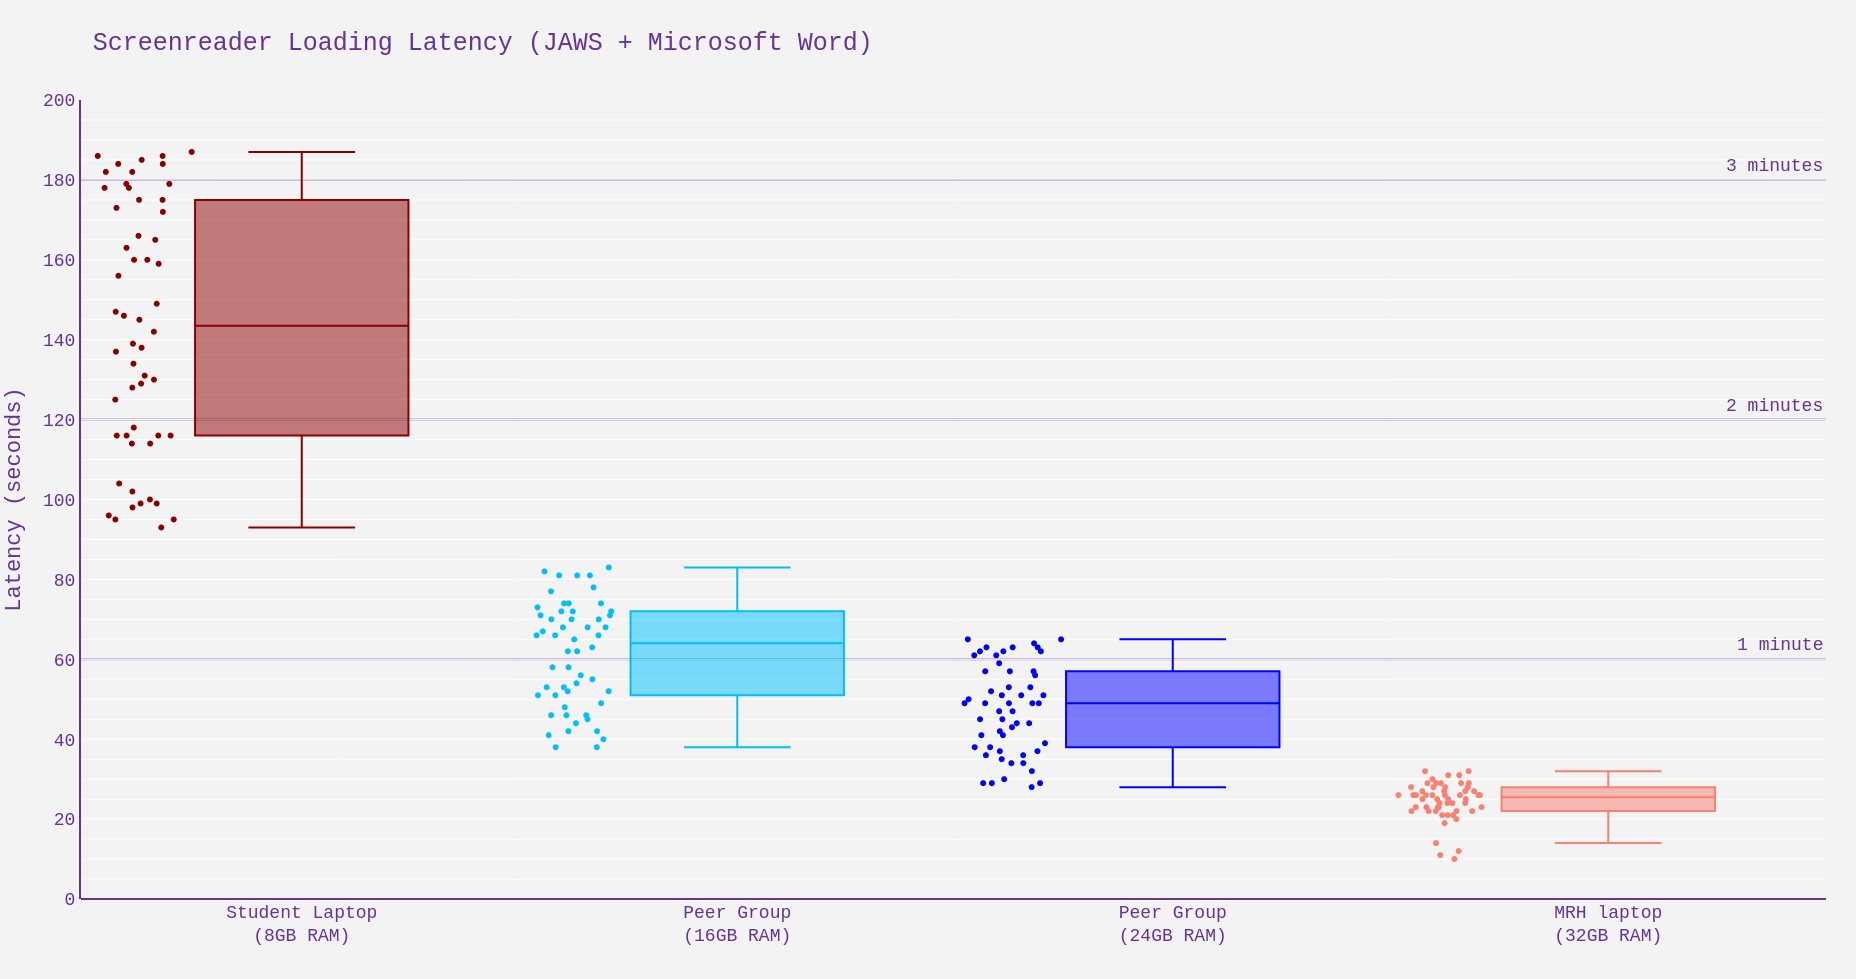
\includegraphics[width=1\linewidth]{images/ComputerRBDisplaySpecsTVIFig1.png}
 \caption[Latency to Load JAWS]{Plot showing Latency to Load JAWS while Microsoft Word is open across a student laptop (Low End - \textit{8GB RAM}), a high quality student laptop (Middle Range - \textit{16GB RAM}), professional laptop (Middle Range - \textit{24 GB RAM}), and a high power laptop (High End - \textit{32 GB RAM}). }
 \label{fig:figre 1}
\end{figure}

\pagebreak \hypertarget{screenreader-response}{%
\subsection*{Screenreader Responsivity}\label{screenreader-response}}
\extramarks{Vision Department Technology Needs}{Screenreader Response}
\addcontentsline{toc}{subsection}{Screenreader Response}

\begin{longtable}[]{@{}
 >{\raggedright\arraybackslash}p{.4\textwidth}
 >{\raggedright\arraybackslash}p{.25\textwidth}
 >{\raggedright\arraybackslash}p{.25\textwidth}
@{}
 }
 
\toprule\noalign{}

\textbf{Computer} \break (Color as Labelled in Figure 1) & \textbf{Loading Time}\break (median [Range]) & \textbf{Response Lag}\break (median [Range])
\\
\midrule\noalign{}
\endhead
\bottomrule\noalign{}
\endlastfoot
\fcolorbox{red}{red}{\rule{0pt}{6pt}\rule{6pt}{0pt}}\qquad $\begin{array}{l}\textbf{Students Laptop} \\ \text{8GB RAM}\end{array}$ & 143 [93-183] \footnote{These are the data plotted in the Figure above} & 38 [27-91]\footnote{It is further important to note here that any lag in screenreader responsiveness of \textgreater1 sec means the student is behind their peers and their educational opportunity is limited by the technology not being sufficient (\emph{i.e.}, not an adequate accommodation). } \\[1.0em] 
\fcolorbox{cyan}{cyan}{\rule{0pt}{6pt}\rule{6pt}{0pt}}\qquad$\begin{array}{l}\textbf{Students Laptop} \\ \text{16GB RAM}\end{array}$ & 64 [38-93] & 9 [4-15] \\[1.0em] 
\fcolorbox{violet}{violet}{\rule{0pt}{6pt}\rule{6pt}{0pt}}\qquad$\begin{array}{l}\textbf{Professional Laptop} \\ \text{24GB RAM}\end{array}$& 49 [26-65] &1 [0.05-2.5] \\[1.0em] 
\fcolorbox{orange}{orange}{\rule{0pt}{6pt}\rule{6pt}{0pt}}\qquad$\begin{array}{l}\textbf{My Personal Laptop} \\ \text{32GB RAM}\end{array}$ & 25 [10-32] &0.5 [0.01-1]\footnote{.01 is for immediate responses that could not be measured} \\ [1.0em] \hline \caption*{ Lag in JAWS Reporting HTML Content} \\
\end{longtable}


\pagebreak \hypertarget{notes-on-future-proofing-laptops}{%
\section*{Laptop Cost Factors}\label{notes-on-future-proofing-laptops}}

\extramarks{Vision Department Technology Needs}{Laptop Cost Analysis}
\addcontentsline{toc}{section}{Laptop Cost Factors}

\hypertarget{notes-on-future-proofing-laptops}{%
\subsection*{Laptop Cost Factors}\label{notes-on-future-proofing-laptops}}
\extramarks{Vision Department Technology Needs}{Laptop Durability}
\addcontentsline{toc}{subsection}{Laptop Durability}

I asked ChatGPT why I should consider future usage needs of a laptop into my purchasing plans and here is its response:

\begin{quote}
Buying laptops with high-end RAM and processor specifications can be beneficial for several reasons, especially in terms of longevity and performance. Here are some key considerations:

\begin{enumerate}
\def\labelenumi{\arabic{enumi}.}

\item
 Future-Proofing:
\end{enumerate}

\begin{itemize}

\item
 Investing in higher-end components can help future-proof your laptop to some extent. As software and applications become more demanding over time, a laptop with better specifications is likely to remain relevant and capable of handling new software updates and requirements.
\end{itemize}

\begin{enumerate}
\def\labelenumi{\arabic{enumi}.}
\setcounter{enumi}{1}

\item
 Multitasking and Performance:
\end{enumerate}

\begin{itemize}

\item
 Higher RAM allows for better multitasking capabilities. If you use resource-intensive applications or run multiple programs simultaneously, having ample RAM prevents slowdowns and ensures smooth performance.
\item
 A powerful processor can handle complex computations and tasks more efficiently, contributing to faster overall system performance.
\end{itemize}

\begin{enumerate}
\def\labelenumi{\arabic{enumi}.}
\setcounter{enumi}{2}

\item
 Graphics Processing:
\end{enumerate}

\begin{itemize}

\item
 For tasks such as video editing, gaming, or other graphics-intensive applications, a high-end GPU (Graphics Processing Unit) is crucial. This is separate from RAM and the main processor but is equally important for certain tasks.
\end{itemize}

\begin{enumerate}
\def\labelenumi{\arabic{enumi}.}
\setcounter{enumi}{3}

\item
 Long-Term Usability:
\end{enumerate}

\begin{itemize}

\item
 Technology advances quickly, and what is considered high-end today might become standard or entry-level in a few years. However, starting with a high-end laptop gives you a more extended period before your system becomes outdated.
\end{itemize}

\begin{enumerate}
\def\labelenumi{\arabic{enumi}.}
\setcounter{enumi}{4}

\item
 Smooth Upgrades:
\end{enumerate}

\begin{itemize}

\item
 Some laptops allow users to upgrade certain components like RAM and storage. Starting with higher-end specifications provides more headroom for future upgrades, allowing you to extend the useful life of your laptop.
\end{itemize}

\begin{enumerate}
\def\labelenumi{\arabic{enumi}.}
\setcounter{enumi}{5}

\item
 Resource-Intensive Applications:
\end{enumerate}

\begin{itemize}

\item
 If you use applications that require a lot of processing power, like video editing software, 3D modeling tools, or virtualization software, a high-end laptop can handle these tasks more efficiently, providing a better user experience.
\end{itemize}

\begin{enumerate}
\def\labelenumi{\arabic{enumi}.}
\setcounter{enumi}{6}

\item
 Responsiveness and Speed:
\end{enumerate}

\begin{itemize}

\item
 A faster processor and more RAM contribute to a more responsive system. Applications load quicker, and the overall user experience is smoother, which can significantly impact productivity.
\end{itemize}

\begin{enumerate}
\def\labelenumi{\arabic{enumi}.}
\setcounter{enumi}{7}

\item
 Enhanced Resale Value:
\end{enumerate}

\begin{itemize}

\item
 High-end laptops generally retain their value better than lower-end models. If you decide to sell or upgrade your laptop in the future, having top-tier specifications can make it more attractive to potential buyers.
\end{itemize}

It's important to note that the specific requirements depend on your usage patterns and needs. Not everyone needs the highest specifications, and sometimes a mid-range laptop can be more than sufficient for everyday tasks. However, for users with demanding workloads or those who want a longer usable life from their device, opting for higher-end specifications can be a wise investment.
\end{quote}

Other than the resale value I agree with all of the reasons given. I am a recycle the computer back to the vendor rather than a sell it to someone that doesn't understand the limitations that are leading me to sell the equipment kind of person.

\pagebreak \hypertarget{optimizing-cost-with-performance}{%
\subsection*{Laptop Cost Optimization}\label{optimizing-cost-with-performance}}

\extramarks{Vision Department Technology Needs}{Laptop Cost Optimization}
\addcontentsline{toc}{subsection}{Laptop Cost Optimization}


There is an economic theory based on a Terry Pratchett novel that explains this phenomenon better than I can. It is called the \href{https://en.wikipedia.org/wiki/Boots_theory}{Boots theory}\footnote{Full Text (emphasis mine): 
\begin{quote}The reason that the rich were so rich, Vimes reasoned, was because they managed to spend less money.

Take boots, for example. He earned thirty-eight dollars a month plus allowances. A really good pair of leather boots cost fifty dollars. But an affordable pair of boots, which were sort of OK for a season or two and then leaked like hell when the cardboard gave out, cost about ten dollars. Those were the kind of boots Vimes always bought, and wore until the soles were so thin that he could tell where he was in Ankh-Morpork on a foggy night by the feel of the cobbles.

But the thing was that good boots lasted for years and years. \textbf{A man who could afford fifty dollars had a pair of boots that’d still be keeping his feet dry in ten years’ time, while the poor man who could only afford cheap boots would have spent a hundred dollars on boots in the same time and would still have wet feet.}

Basically, \textbf{we are destined to be stuck in a cycle of perpetually spending more money for inferior products and will, in the end, spend more money than if we just paid for better product in the first place.}
\end{quote} }

\hfill \break Here is this economic theory illustrated in terms of student laptop computers (Assuming student has a laptop through 3rd-12th grade).

\hspace{-1cm}\begin{longtable}[]{@{}
 >{\raggedright\arraybackslash}p{.15\textwidth}
 >{\raggedright\arraybackslash}p{.05\textwidth}
 >{\raggedright\arraybackslash}p{.05\textwidth}
 >{\raggedright\arraybackslash}p{.05\textwidth}
 >{\raggedright\arraybackslash}p{.05\textwidth}
 >{\raggedright\arraybackslash}p{.05\textwidth}
 >{\raggedright\arraybackslash}p{.05\textwidth}
 >{\raggedright\arraybackslash}p{.05\textwidth}
 >{\raggedright\arraybackslash}p{.05\textwidth}
 >{\raggedright\arraybackslash}p{.05\textwidth}
 >{\raggedright\arraybackslash}p{.05\textwidth}
 >{\raggedright\arraybackslash}p{.10\textwidth}@{}
 }
\toprule\noalign{}
 & 
\multicolumn{10}{c}{\textbf{Does School Have to Purchase a Replacement Laptop by Year}} & \\
\cline{2-11} \\
\textbf{RAM} \break \textbf{Cost} &
\textbf{1} & 
\textbf{2} & 
\textbf{3} & 
\textbf{4} & 
\textbf{5} & 
\textbf{6} & 
\textbf{7} & 
\textbf{8} & 
\textbf{9} & 
\textbf{10} & 
\textbf{Total Cost}\\
\midrule\noalign{}
\endhead
\bottomrule\noalign{}
\endlastfoot
\textbf{8GB} \break \$1000\footnote{The \emph{Low End Laptop} is the mean of what I am seeing online right now (range \$750-\$1250). Importantly, I cannot use the current student laptops for this example as they are incapable of running JAWS concurrently with any other programs} & $\checkmark$ & $\checkmark$ & $\checkmark$& $\checkmark$ & $\checkmark$ & $\checkmark$ & $\checkmark$ & $\checkmark$ & $\checkmark$ & $\checkmark$ & \$10,000 \\[2.0em]
\textbf{16GB} \break \$1751\footnote{The \emph{Mid Range} Laptop is the current Dell Precision 3530 given to TVI teaching screenreaders} & $\checkmark$ & -- & $\checkmark$ & -- & $\checkmark$ & -- & $\checkmark$& -- & $\checkmark$ & -- & \$8,755 \\[2.0em]
\textbf{32GB}\break \$2824\footnote{The \emph{High End Laptop} here is my personal Microsoft Surface Laptop 3, and the update price reflects an update to the Surface 5 with current prices} & $\checkmark$ & -- & -- & -- & -- & $\checkmark$ & -- & -- & -- & -- & \$5,648 \\[2.0em] \hline
 \caption{ Cost of Laptops over Time}
\end{longtable}


I put this Table here to illustrate why I choose to err on the side of spending \$2000-3000 now on a laptop that will last 3-5 years over spending \$1500-2000 on a laptop that will barely make it 1-2 years before becoming obsolete. By the end of 5 years I will have spent more on Low End and Mid Range Laptops than I would have had I purchased a High End Laptop. Importantly; however, I also would have been using laptops that always perform more poorly than a High End laptop would.

\pagebreak \hypertarget{minimum-laptop-recommendations}{%
\section*{Recommended Laptop Specifications}\label{minimum-laptop-recommendations}}
\extramarks{Vision Department Technology Needs}{Recommended Laptop Specifications}

\emph{Organized by Usage Case}

\begin{itemize}
\item
 Screenreader Only (No magnification or monitor modifications needed)

 \begin{itemize}
 
 \item
 JAWS Screenreader while running Microsoft Word, a browser, and Powerpoint (situation typical for in 5-12th grade): \textbf{24-32GB}
 \end{itemize}
\item
 Screenreader + Magnification (Laptop needs a \textbf{monitor with Screen Size \textgreater15 inches}; does \emph{not} need to be a touchscreen)

 \begin{itemize}
 
 \item
 JAWS Screenreader + Windows Magnifier while running Microsoft Word, a browser, and Powerpoint(typical for 5-12th grade): \textbf{24-32GB}
 \item
 SuperNova Screenreader + Magnification while running Microsoft Word, a browser, and Powerpoint(typical for 5-12th grade): \textbf{32-64GB}
 \item
 Fusion Screenreader + Magnification while running Microsoft Word, a browser, and Powerpoint(typical for 5-12th grade): \textbf{32-64GB}
 \end{itemize}
\end{itemize}

\pagebreak \hypertarget{laptop-options}{%
\chapter*{Laptop Options}\label{laptop-options}}

\hypertarget{laptops-meeting-redcommended-specifications}{%
\section*{Laptops Meeting Recommended
Specifications}\label{laptops-meeting-redcommended-specifications}}

\extramarks{Vision Department Technology Needs}{Laptops Meeting Recommended
Specifications}
\addcontentsline{toc}{subsection}{Laptops Meeting Recommended Specifications}

\begin{longtable}[]{@{}
 >{\raggedright\arraybackslash}p{.3\textwidth}
 >{\raggedright\arraybackslash}p{.1\textwidth}
 >{\raggedright\arraybackslash}p{.05\textwidth}
 >{\raggedright\arraybackslash}p{.1\textwidth}
 >{\raggedright\arraybackslash}p{.05\textwidth}
 >{\raggedright\arraybackslash}p{.1\textwidth}
 >{\raggedright\arraybackslash}p{.2\textwidth}@{}
 }
\toprule\noalign{}

\textbf{Company / Model}
& 
\textbf{Cost}
& 
\textbf{Battery}
& 
\textbf{Keyboard}
& 
\textbf{RAM}
& 
\textbf{Screen Size}
& 
\textbf{Processor}
\\
\midrule\noalign{}
\endhead
\bottomrule\noalign{}
\endlastfoot
Framework 13 & \$1,102 & 60W & QWERTY & 32GB & 13.5'' & 13th Gen i7 \\
Framework 13 & \$2,222 & 60W & QWERTY & 64GB & 13.5'' & 13th Gen i7 \\
Framework 13 & \$1,732 & 60W & QWERTY & 32GB & 13.5'' & AMD Ryzen 7 \\
Framework 13 & \$1,892 & 60W & QWERTY & 64GB & 13.5'' & AMD Ryzen 7 \\
Framework 16 & \$2,239 & 180W & QWERTY\break (+NUMPAD) & 32GB & 16'' & AMD Ryzen 9 \\
Framework 16\break (+ AMD GPU) & \$2,639 & 180W & QWERTY\break (+NUMPAD) & 32GB & 16'' & AMD Ryzen 9 \\
Framework 16 & \$2,399 & 180W & QWERTY\break (+NUMPAD) & 64GB & 16'' & AMD Ryzen 9 \\
Framework 16\break (+ AMD GPU) & \$2,799 & 180W & QWERTY\break (+NUMPAD) & 64GB & 16'' & AMD Ryzen 9 \\
Dell Precision 5770 & \$2,789 & 97W & QWERTY & 32GB & 17'' & 12th Gen i7 \\
Dell XPS 15 & \$2,099 & 97W & QWERTY & 32GB & 15.6''\break Touchscreen & 12th Gen i7 \\
Dell XPS 15 & \$2,349 & 97W & QWERTY & 32GB & 15.6''\break Touchscreen & 12th Gen i9 \\
Dell XPS 15 & \$2,999 & 97W & QWERTY & 32GB & 15.6''\break Touchscreen & 13th Gen i9 \\
Dell XPS 17 & \$3,349 & 97W & QWERTY & 32GB & 15.6''\break Touchscreen & 13th Gen i7 \\
Dell XPS 17 & \$3,549 & 97W & QWERTY & 32GB & 15.6''\break Touchscreen & 13th Gen i9 \\
Alienware m16 Gaming Laptop & \$3,499 & 97W & QWERTY & 32GB & 16.0'' & 13th Gen 19 \\
Alienware x14 Gaming Laptop & \$1,999 & 97W & QWERTY & 32GB & 14.0'' & 13th Gen i7 \\
Dell XPS 13 Plus & \$2,009 & 97W & QWERTY & 32GB & 13.4'' & 13th Gen i7 \\
Dell latitude 7440 & \$3,615 & 97W & QWERTY & 32GB & 14.0'' & 13th Gen i7 \\
Dell G16 Gaming Laptop & \$1,999 & 97W & QWERTY & 32GB & 16.0'' & 13th Gen i7 \\
Dell precision 5680 & \$5,597 & 97W & QWERTY & 32GB & 16.0'' & 13th Gen i9 \\
Dell Inspiron 16 Plus & \$1,499 & 97W & QWERTY & 32GB & 16.0'' & 13th Gen i7 \\
Dell precision 7680 & \$7,225 & 97W & QWERTY & 32GB & 16.0'' & 13th Gen i9 \\
Dell Precision 5480 & \$4,354 & 97W & QWERTY & 32GB & 14.0'' & 13th Gen i7 \\
Dell Precision 3480 & \$3,205 & 97W & QWERTY & 32GB & 14.0'' & 13th Gen i7 \\
Dell Precision 3581 & \$3,854 & 97W & QWERTY & 32GB & 15.6'' & 13th Gen i7 \\
HP Dragonfly Pro & \$1,549 & 97W & QWERTY & 32GB & 14.0''\break Touchscreen & AMD Ryzen 7 \\
HP Envy & \$1,749 & 97W & QWERTY & 32GB & 17.3'' & 13th Gen i7 \\
Acer Predator Helios 16 & \$2,499 & 97W & QWERTY & 32GB & 16.0'' & 13th Gen i9 \\
Acer Predator Triton & \$3,799 & 97W & QWERTY & 64GB & 17.0'' & 13th Gen i9 \\
Asus ProArt Studiobook & \$2,999 & 97W & QWERTY & 32GB & 16.0'' & 13th Gen i9 \\
Asus Zenbook Pro 16X & \$2,599 & 97W & QWERTY & 32GB & 16.0'' & 13th Gen i9 \\
MSI Vector & \$1,999 & 97W & QWERTY & 64GB & 14.0'' & 13th Gen i9 \\
Lenovo Thinkpad P14s & \$2,509 & 97W & QWERTY & 64GB & 14.0'' & AND Ryzen 7 \\
Lenovo Thinkpad P14s & \$2,199 & 97W & QWERTY & 32GB & 14.0'' & AND Ryzen 7 \\
Legion Pro 7i & \$3,599 & 97W & QWERTY & 32GB & 16.0'' & 13th Gen i9 \\
Lenovo Thinkpad X1 Yoga & \$3,719 & 97W & QWERTY & 32GB & 14.0'' & 13th Gen i7 \\
Lenovo ThinkPad P16v & \$3,339 & 65W & QWERTY & 32GB & 16'' & 13th Gen i7 \\
Lenovo ThinkPad P16v & \$4,929 & 65W & QWERTY & 64GB & 16'' & 13th Gen i7 \\
Lenovo ThinkPad P16 Gen 2 & \$3,239 & 65W & QWERTY & 32GB & 16'' & 13th Gen i7 \\
Lenovo ThinkPad P16 Gen 2 & \$4,189 & 65W & QWERTY & 64GB & 16'' & 13th Gen i7 \\
Lenovo ThinkPad P16 Gen 2 & \$4,829 & 65W & QWERTY & 64GB & 16'' & 13th Gen i7 \\
Lenovo ThinkPad P16 Gen 2 & \$2,039 & 65W & QWERTY & 32GB & 16'' & AMD Ryzen 7 \\
Lenovo ThinkPad P16 Gen 2 & \$2,829 & 65W & QWERTY & 64GB & 16'' & AMD Ryzen 7 \\
Microsoft Surface Laptop 5 & \$2824.97 & 97W & QWERTY & 32GB & 15''\break Touchscreen & 12th Gen i7 \\
Orbit Optima & \$3,000-\$6,000 & TBD & QWERTY & 16GB-64GB & none & 13th Gen i7 \\
Nattiq Note & \$4,225-\$5,200 & 97W & QWERTY & 4GB-32GB & none & 12th Gen i7 \\
Notey the Notetaker & \textasciitilde\$750+\footnote{Self build
\href{https://notey-project.com/2023/03/07/notey-user-manual-v1-0-2/}{Specs
for Notey the NoteTaker}} &
60W & QWERTY \break Perkins & 8GB-16GB & none & Celeron
N5105 \\ [1.0em] \hline
\caption{ Laptop Options}
\end{longtable}

\pagebreak \hypertarget{braille-first-devices}{%
\chapter*{Braille First Devices}\label{braille-first-devices}}
\extramarks{Vision Department Technology Needs}{Braille Devices}
\addcontentsline{toc}{chapter}{Braille Devices}

\hypertarget{braille-notetakers-and-braille-laptop-computers}{%
\section*{Braille Notetakers and Laptops}\label{braille-notetakers-and-braille-laptop-computers}}
\extramarks{Vision Department Technology Needs}{Braille Notetakers and Laptops}
\addcontentsline{toc}{subsection}{Braille Notetakers and Laptops}

\begin{longtable}[]{@{}
 >{\raggedright\arraybackslash}p{.12\textwidth}
 >{\raggedright\arraybackslash}p{.08\textwidth}
 >{\raggedright\arraybackslash}p{.08\textwidth}
 >{\raggedright\arraybackslash}p{.08\textwidth}
 >{\raggedright\arraybackslash}p{.05\textwidth}
 >{\raggedright\arraybackslash}p{.08\textwidth}
 >{\raggedright\arraybackslash}p{.12\textwidth}
 >{\raggedright\arraybackslash}p{.12\textwidth}@{}
 }
\toprule\noalign{}

\textbf{Display}
& 
\textbf{Cost}
& 
\textbf{Battery}
& 
\textbf{Memory}
&
\textbf{Files Types}
&
\textbf{Keyboard}
&
\textbf{Manufacturer}
&
\textbf{OS}
\\
\midrule\noalign{}
\endhead
\bottomrule\noalign{}
\endlastfoot
Orbit Optima & \$6,000 & TBD & 16GB - 64GB & all & QWERTY & Orbit Research & Windows 11 \\[1.0em]
BrailleNote Touch+\footnote{For both the BrailleNote Touch+ and BrailleSense 6, there is an emerging issue with outdated operating systems, WiFi connectivity inconsistencies, and incompatibility with Google applications. \begin{itemize}
\item
 \href{https://perkins.org/braillenote-touch-outdated-os/}{Link to article from Perkins.org regarding the BrailleNote Touch Plus}
\item
 \href{https://endoflife.date/android}{Continually Updated List for End of Life for all flavors of AndroidOS}
\end{itemize}} & \$5,795 & 12h & 64GB & docx, brf, ePub, DAISY & Perkins & Humanware & Android 8\footnote{Android 8 `Oreo' Security Support Ended (\emph{i.e.}, End of Life) 2017-12-05} \\[1.0em]
BrailleSense 6 & \$5,795 & 12h & 128GB & docx, brf, ePub, DAISY & Perkins & HIMS & Android 10\footnote{Android 10 `Queen Cake' Security Support Ended (\emph{i.e.}, End of Life) 2023-03-06}\footnote{The Braillesense has a firmware update v2.0 released 2023-11-28 which updates the operating system to Android 12, but this is currently buggy and causing system overheating. (\emph{note:} Android 12 will only receive updates until \textasciitilde October of 2024)} \\[1.0em]
InsideONE & \$5,499 & 6h & 128GB & all & Perkins & InsideVision & Windows 11 \\[1.0em]
Nattiq Note & \$5,200 & 12h & 4GB - 32GB & all & QWERTY & Nattiq & Windows 11 \\[1.0em]
Notey the Notetaker & \textasciitilde\$750+\footnote{Self build
\href{https://notey-project.com/2023/03/07/notey-user-manual-v1-0-2/}{Specs for Notey the NoteTaker}} & & 8GB - 16GB & all & QWERTY Perkins & Miscs & Windows 11 \\[1.0em]
b.note & \$4,360 & 15h & SD 64GB & all & Perkins & Eurobraille & Proprietary \\[1.0em]\hline
\caption{ Braille NoteTakers and Laptops }
\end{longtable}
\addcontentsline{toc}{section}{ Braille NoteTakers and Laptops }

\pagebreak \hypertarget{cell-refreshable-braille-displays}{%
\section*{32-40 cell Refreshable Braille
Displays}\label{cell-refreshable-braille-displays}}
\extramarks{Vision Department Technology Needs}{32-40 cell Refreshable Braille
Displays}
\addcontentsline{toc}{subsection}{32-40 cell Refreshable Braille Displays}

\begin{longtable}[]{@{}
 >{\raggedright\arraybackslash}p{.15\textwidth}
 >{\raggedright\arraybackslash}p{.05\textwidth}
 >{\raggedright\arraybackslash}p{.08\textwidth}
 >{\raggedright\arraybackslash}p{.08\textwidth}
 >{\raggedright\arraybackslash}p{.15\textwidth}
 >{\raggedright\arraybackslash}p{.12\textwidth}
 >{\raggedright\arraybackslash}p{.15\textwidth}@{}
 }
\toprule\noalign{}

Display & Cost & Battery & Memory & File Types & Keyboard & Manufacturer \\
\midrule\noalign{}
\endhead
\bottomrule\noalign{}
\endlastfoot
Brailliant BI40x & \$3,195 & 14 & 32GB & brf, txt, docx, pdf, DAISY, zip & Perkins & Humanware \\[1.0em]
Focus 40 Blue & \$3,145 & 18 & microSD & brf, txt & Perkins & Vispero \\[1.0em] Mantis Q40 & \$2,495 & 14 & 16GB & brf, txt, docx, DAISY, zip & QWERTY & APH\break Humanware \\[1.0em]
Orbit Reader 40 & \$1,399 & 20 & SD Card & brf, txt & Perkins & Orbit Research \\[1.0em]
QBraille XL & \$3,195 & 16 & SD Card & brf, txt, rtf, docx, PDF & Perkins & HIMS \\[1.0em]
Basic Braille Plus & \$3,295 & 12 & n/a & n/a & Perkins & Help Tech \\[1.0em] Active Star & \$6,795 & 40 & 16GB & doc, docx, rtf, txt, brf, brl, xls, xlsx, PDF & Perkins & Help Tech \\[1.0em]
Active Braille & \$6,495 & 20 & 64GB & doc, docx, rtf, txt, brf, brl, xls, xlsx, PDF & Perkins & Help Tech \\[1.0em]
Activator & \$6,495 & 40 & 64GB & doc, docx, rtf, txt, brf, brl, xls, xlsx, PDF & Perkins\break QWERTY & Help Tech \\[1.0em]
Vario Ultra 40 & \$7,643 & 12 & USB, 32GB & doc, docx, rtf, txt, brf, brl, xls, xlsx, PDF & Perkins & VisioBraille \\[1.0em]
Vario 340 & \$5,138 & 20 & n/a & n/a & none & VisioBraille \\[1.0em]
Vario 440 & \$4,550 & 20 & n/a & n/a & none & VisioBraille \\[1.0em]
Seika V5 & \$2,495 & 20 & 4GB & brf, txt & none & Nippon Telesoft \\[1.0em]
Alva 640 Comfort & \$3,046 & 10 & 8GB & brf & Perkins & Optelec \\[1.0em]
Alva 640 USB & \$3837 & n/a & n/a & n/a & none & Optelec \\[1.0em]
Alva BC 640 & \$2,087 & 10 & 4GB & n/a & none & Alva \\[1.0em]
b.note & \$3,565 & 15 & 64GB & doc, docx, rtf, txt, brf, brl, xls, xlsx, PDF & Perkins & Eurobraille \\[1.0em] \hline
\caption{ 32-40 cell Single Line Refreshable Braille Displays }
\end{longtable}

\pagebreak \hypertarget{multiple-line-refreshable-braille-displaystablets}{%
\section*{Multiple Line Refreshable Braille Displays/Tablets}\label{multiple-line-refreshable-braille-displaystablets}}

\extramarks{Vision Department Technology Needs}{Multiple Line Refreshable Braille
Displays/Tablets}
\addcontentsline{toc}{subsection}{Multiple Line Refreshable Braille Displays/Tablets}

\begin{longtable}[]{@{}
 >{\raggedright\arraybackslash}p{.2\textwidth}
 >{\raggedright\arraybackslash}p{.1\textwidth}
 >{\raggedright\arraybackslash}p{.1\textwidth}
 >{\raggedright\arraybackslash}p{.15\textwidth}
 >{\raggedright\arraybackslash}p{.15\textwidth}
 >{\raggedright\arraybackslash}p{.15\textwidth}@{}
 }
\toprule\noalign{}

\textbf{Display}
&
\textbf{Cost}
&
\textbf{Battery}
&
\textbf{Braille Lines}
&
\textbf{Keyboard}
&
\textbf{Manufacturer}
\\
\midrule\noalign{}
\endhead
\bottomrule\noalign{}
\endlastfoot
Orbit Slate 520 & \$3,495 & 20-22 & 5 row x 20 cell & Perkins & Orbit Research \\[1.0em]
Orbit Slate 340 & \$3,995 & 20-22 & 5 row x 20 cell & Perkins & Orbit Research \\[1.0em]
Graphiti & \textasciitilde\$15,000 & 20-22 & 60 row x 40 cell & Perkins & Orbit Research \\[1.0em]
Graphiti Plus & \textasciitilde\$15,000 & 20-22 & 60 row x 40 cell + 40 cell line & Perkins & Orbit Research \\[1.0em]
TACTIS Table & \textasciitilde\$15,000 - \$20,000 & Requires AC & 25 row x 40 cell & none & Tactisplay \\[1.0em]
TACTIS Walk & \textasciitilde\$7,000 & Requires AC & 10 row x 25 cell & none & Tactisplay \\[1.0em]
TACTIS 100 & \textasciitilde\$5,000 & Requires AC & 4 row x 25 cell & none & Tactisplay \\[1.0em]
Canute 360 & \$2,895 & Requires AC & 9 row x 40 cell & none & Bristol Braille \\[1.0em]
DotPad\break (Apple/iOS) & \textasciitilde\$13,000-\$18,000 & 11 hr & 10 row x 32 cell + 20 cell line & Touch interface & Dot Inc. \\[1.0em]
APH Monarch\break (Apple/iOS/Windows) & \textasciitilde\$13,000-\$18,000 & 11 hr & 10 row x 32 cell line & Perkins & Dot Inc.\break Humanware\break APH \\[1.0em]
Blitab & \$500 & TBD & 14 row x 23 cell & Touch Interface & Blitab \\[1.0em]
Tactile Pro & TBD & TBD & TBD & Perkins & PCT \\[1.0em]
NewHaptics (?) & TBD & TBD & TBD & TBD & New Haptics \\[1.0em]
InsideONE & \$5,499 & 6h & 128GB & Perkins & InsideVision \\[1.0em]
BraillePad & \$4,390 & ? & 50 row x 40 cells & none & 4Blind \\[1.0em]
Cadence & TBD & ? & 6 row x 8 cells stack to 24 x 16 & Perkins & Tactile Engineering \\[1.0em]
Tactonom Pro & \textasciitilde\$15,000 & Requries AC & 119 col x 89 lines 10,500 touch points & N/A & Tactonom \\[1.0em]\hline
\caption{ Multiple Line Refreshable Braille Devices }
\end{longtable}


\pagebreak \hypertarget{generation}{%
\chapter*{Braille Generation}\label{generation}}
\extramarks{Vision Department Technology Needs}{Braille Generation}
\addcontentsline{toc}{chapter}{Braille Generation}

\pagebreak \hypertarget{embossers}{%
\section*{Braille Embossers}\label{embossers}}
\extramarks{Vision Department Technology Needs}{Braille Embossers}
\addcontentsline{toc}{section}{Braille Embossers}

\begin{longtable}[]{@{}
 >{\raggedright\arraybackslash}p{.2\textwidth}
 >{\raggedright\arraybackslash}p{.1\textwidth}
 >{\raggedright\arraybackslash}p{.4\textwidth}
 >{\raggedright\arraybackslash}p{.15\textwidth}@{}
 }
\toprule\noalign{}

\textbf{Machine}
&
\textbf{Cost}
&
\textbf{Capability}
&
\textbf{Company}
\\
\midrule\noalign{}
\endhead
\bottomrule\noalign{}
\endlastfoot
ViewPlus Rogue\break (used to be Max) & \$5,995 & Complex Graphics, Interpoint Braille & ViewPlus \\[1.0em]
ViewPlus Columbia & \$3,495 & Complex Graphics, Interpoint Braille & ViewPlus \\[1.0em]
APH PageBlaster\break (old Model Index-D V4) & \$4,295\footnote{Requires free \href{https://www.aph.org/app/uploads/2020/07/Firebird_signed_V31.zip}{Firebird Tactile Graphics} Software for graphics functionality} & Simple Graphics, Interpoint Braille & APH\break Index Braille \\[1.0em]
Basic-D V5 & \$3,695\footnote{Requires \href{https://tactileview.com/}{TactileView} license for full graphics functionality (\$\$484 for 1 year seat license)} & Simple Graphics, Interpoint Braille & Index Braille \\[1.0em]
Juliet 120 & \$4,195\footnote{Requires free \href{https://www.aph.org/app/uploads/2020/07/Firebird_signed_V31.zip}{Firebird Tactile Graphics} Software for graphics functionality} & Simple Graphics, Interpoint Braille & ETS\break Humanware \\[1.0em]
BrailleTrac 120 & \$3,595 & Simple Graphics, Interpoint Braills & Irie-AT \\[1.0em]\hline
\caption{ Braille Embossers focusing on Text}
\end{longtable}


\pagebreak \hypertarget{tactile-graphics-high-resolution-complex-graphics}{%
\section*{Tactile graphics (High Resolution Graphics)}\label{tactile-graphics-high-resolution-complex-graphics}}

\extramarks{Vision Department Technology Needs}{Tactile Graphics (High Resolution
Graphics)}
\addcontentsline{toc}{section}{Tactile Graphics (High Resolution
Graphics)}

\begin{longtable}[]{@{}
 >{\raggedright\arraybackslash}p{.5\textwidth}
 >{\raggedright\arraybackslash}p{.3\textwidth}
 >{\raggedright\arraybackslash}p{.15\textwidth}@{}
 }
\toprule\noalign{}

\textbf{Machine} & \textbf{Cost} & \textbf{Company} \\
\midrule\noalign{}
\endhead
\bottomrule\noalign{}
\endlastfoot
PIAF tactile embosser & \$1,745 & Humanware \\[1.0em]
Swell Form Machine & \$1,400.00 & American Thermoform \\[1.0em]
EZ-Form Brailon Duplicator & \$3,899 & American thermoform \\[1.0em]
ViewPlus Rogue \break (used to be ViewPlus Max) & \$5,995\footnote{Requires \href{https://viewplus.com/product/tiger-software-suite8/}{Tiger Software Suite} for full functionality (\$195 for 1 year seat license; \$595 for perpetual seat license)} & ViewPlus \\[1.0em]
ViewPlus Columbia & \$3,495\footnote{Requires \href{https://viewplus.com/product/tiger-software-suite8/}{Tiger Software Suite} for full functionality (\$195 for 1 year seat license; \$595 for perpetual seat license)} & ViewPlus \\[1.0em]
APH PixBlaster \break (old Model ViewPlus Columbia) & \$4,295\footnote{Requires \href{https://viewplus.com/product/tiger-software-suite8/}{Tiger Software Suite} for full functionality (\$195 for 1 year seat license; \$595 for perpetual seat license)} & APH\break ViewPlus \\[1.0em]
ViewPlus Delta & \$4,195\footnote{Requires \href{https://viewplus.com/product/tiger-software-suite8/}{Tiger Software Suite} for full functionality (\$195 for 1 year seat license; \$595 for perpetual seat license)} & ViewPlus \\[1.0em]
ViewPlus Premier & \$9,995\footnote{Requires \href{https://viewplus.com/product/tiger-software-suite8/}{Tiger Software Suite} for full functionality (\$195 for 1 year seat license; \$595 for perpetual seat license)} & ViewPlus \\[1.0em]
ViewPlus Elite & \$14,995\footnote{Requires \href{https://viewplus.com/product/tiger-software-suite8/}{Tiger Software Suite} for full functionality (\$195 for 1 year seat license; \$595 for perpetual seat license)} & ViewPlus \\[1.0em]
Basic-D V5 & \$3,695\footnote{Requires \href{https://tactileview.com/}{TactileView} license for full graphics functionality (\$484 for 1 year seat license)} & Index Braille \\[1.0em]\hline \caption{ Equipment for Tactile Graphics Generation}
\end{longtable}



\hypertarget{tactile-paper}{%
\subsection*{Tactile Graphic Supplies}\label{tactile-paper}}

\extramarks{Vision Department Technology Needs}{Tactile Graphic Supplies}
\addcontentsline{toc}{subsection}{Tactile Graphic Supplies}

\begin{longtable}[]{@{}
 >{\raggedright\arraybackslash}p{.5\textwidth}
 >{\raggedright\arraybackslash}p{.3\textwidth}
 >{\raggedright\arraybackslash}p{.15\textwidth}@{}
 }
\toprule\noalign{}

\textbf{Paper / Medium} & \textbf{Cost} & \textbf{Company} \\
\midrule\noalign{}
\endhead
\bottomrule\noalign{}
\endlastfoot
Tangible Magic capsule Paper (11x11.5'')\break(for PIAF tactile embosser) & \$220 for 100 pages & Humanware \\[1.0em]
Swell Touch Paper \break (for Swell Form Machine) & \$165 for 100 pages & American Thermoform \\[1.0em]
Tractor-Feed Braille Transcribing Paper: (11x11.5'')\break (for embossers) & \$79.47 for 1000 pages & APH \\[1.0em]
Brailon Thermoform Paper\break (for EZ-Form Duplicator) & \$42.99 (100 sheets heavy), \$75.99 (500 sheets regular) & American Thermoform \\[1.0em]\hline
\caption{ Paper supplies for Tactile Graphics Generation }
\end{longtable}


\pagebreak \hypertarget{d-printers}{%
\chapter*{3D Printing}\label{d-printers}}
\extramarks{Vision Department Technology Needs}{3D Printing}
\addcontentsline{toc}{chapter}{3D Printing}
\pagebreak \hypertarget{d-print-equipment}{%
\section*{3D Printers}\label{d-print-equipment}}

\extramarks{Vision Department Technology Needs}{3D Printers}
\addcontentsline{toc}{section}{3D Printers}

\begin{longtable}[]{@{}
 >{\raggedright\arraybackslash}p{.2\textwidth}
 >{\raggedright\arraybackslash}p{.08\textwidth}
 >{\raggedright\arraybackslash}p{.2\textwidth}
 >{\raggedright\arraybackslash}p{.2\textwidth}
 >{\raggedright\arraybackslash}p{.2\textwidth}@{}
 }
\toprule\noalign{}

\textbf{Model}
&
\textbf{Cost}
&
P\textbf{rint Bed Size}
&
\textbf{Filament Size}
&
\textbf{Manufacturer}
\\
\midrule\noalign{}
\endhead
\bottomrule\noalign{}
\endlastfoot
Neptune 4 Pro & \$330 & 225x225x265mm & 1.75mm & Elegoo \\[1.0em]
Neptune 3 Max & \$470 & 420x420x500mm & 1.75mm & Elegoo \\[1.0em]
M5C & \$399 & 220x220x250mm & 1.75mm & AnkerMake \\[1.0em]
Kobra Plus & \$499 & 300x300x350mm & 1.75mm & Anycubic \\[1.0em]
Kobra Max & \$569 & 450x400x400mm & 1.75mm & Anycubic \\[1.0em]
Ender 3 Max Neo & \$359 & 300x300x320mm & 1.75mm & Creality \\[1.0em]
Ender 5 Plus & \$579 & 350x350x400mm & 1.75mm & Creality \\[1.0em]
Mini+ & \$459 & 180x180x180mm & 1.75mm & Prusa \\[1.0em]
Sidewinder X2 & \$399 & 300x300x396mm & 1.75mm & Artillery \\[1.0em]
P1P 3D Printer & \$699 & 256×256×256mm & 1.75mm & Bambu \\[1.0em]
P1S 3D Printer & \$949 & 256×256×256mm & 1.75mm & Bambu \\[1.0em]\hline
\caption{ 3D Printers }
\end{longtable}


\hypertarget{d-printer-materials}{%
\subsection*{3D Printer Materials}\label{d-printer-materials}}

\extramarks{Vision Department Technology Needs}{3D Printer Materials}
\addcontentsline{toc}{section}{3D Printer Materials}

\begin{longtable}[]{@{}
 >{\raggedright\arraybackslash}p{.2\textwidth}
 >{\raggedright\arraybackslash}p{.2\textwidth}
 >{\raggedright\arraybackslash}p{.6\textwidth}@{}
 }
\toprule\noalign{}
Item & Cost & Vendor \\
\midrule\noalign{}
\endhead
\bottomrule\noalign{}
\endlastfoot
1.75mm filament & \textasciitilde\$12.00/kg & Elegoo (via Amazon) \\[1.0em]\hline
\caption{ 3D Printer Materials }
\end{longtable}


\pagebreak \hypertarget{low-vision}{%
\chapter*{Low Vision Equipment}\label{low-vision}}
\extramarks{Vision Department Technology Needs}{Low Vision Equipment}
\addcontentsline{toc}{chapter}{Low Vision Equipment}

\hypertarget{video-magnification-devices}{%
\section*{Video Magnification
Devices}\label{video-magnification-devices}}
\extramarks{Vision Department Technology Needs}{Video Magnification Devices}
\addcontentsline{toc}{section}{Video magnification Devices}

\begin{longtable}[]{@{}
 >{\raggedright\arraybackslash}p{.25\textwidth}
 >{\raggedright\arraybackslash}p{.15\textwidth}
 >{\raggedright\arraybackslash}p{.25\textwidth}
 >{\raggedright\arraybackslash}p{.2\textwidth}@{}
 }
\toprule\noalign{}

\textbf{Model}
&
\textbf{Cost}
&
\textbf{Deployment}
&
\textbf{Company}
\\
\midrule\noalign{}
\endhead
\bottomrule\noalign{}
\endlastfoot
Tactonum Pro & £10,000 & Desktop\break Not Readily Mobile\break Requries mobile App & Tactonum \\[1.0em]
Taxtonum Reader & £3,795.00 & Desktop\break Not Readily Mobile & Tactonum \\[1.0em]
MATT Connect v2 & \$3,895 & Desktop\break (Camera + Android Tablet)\break Mobile, but heavy & APH \\[1.0em]
Juno & \$1,392 & Hand-Held (7'' screen) & APH \\[1.0em]
Jupiter Portable Magnifier & \$3,599.00 & Desktop\break Mobile, but heavy & APH \\[1.0em]
ONYX Desk set HD & \$3,330 & Desktop & Freedom Scientific \\[1.0em]
ONYX OCR & \$4,520 & Desktop & Freedom Scientific \\[1.0em]
RUBY & \$600.60 & Hand-Held (4.3'' screen) & Freedom Scientific \\[1.0em]
RUBY 10 & \$1,640 & Hand-Held (10'' Screen) & Freedom Scientific \\[1.0em]
RUBY 7 HD & \$1,317.75 & Hand-Held (7'' Screen) & Freedom Scientific \\[1.0em]
RUBY HD & \$710.85 & Hand-Held (4.3'' screen) & Freedom Scientific \\[1.0em]
RUBY XL HD & \$987.00 & Hand-Held (5'' screen) & Freedom Scientific \\[1.0em]
TOPAZ XL HD & \$4,045.00 & Desktop & Freedom Scientific \\[1.0em]
TOPAZ OCR & \$4,640.00 & Desktop & Freedom Scientific \\[1.0em]
TOPAZ EZ HD & \$3,081.75 & Desktop & Freedom Scientific \\[1.0em]
MAGNA 5 & \$249 & Hand-Held (5'' screen) & Orbit Research \\[1.0em]
MAGNA 4 & \$199 & Hand-Held (4.3'' screen) & Orbit Research \\[1.0em]
MAGNA 3 & \$149 & Hand-Held (3.5'' screen) & Orbit Research \\[1.0em]
I-See 22'' & \$2,095 & Desktop & Irie AT \\[1.0em]
MagniLink Vision & \$3,190 - \$4,250 & Desktop & Irie AT \\[1.0em]
MagniLink One & \$2,395 & Desktop & Irie AT \\[1.0em]
Acuity 22 & \$2,695 & Desktop & Irie AT \\[1.0em]
Acuity 22 Speech & \$3,695 & Desktop & Irie AT \\[1.0em]
Snow 12 & \$1,395 & Desktop\break Mobile & Zoomax \\[1.0em]
Luna 6 & \$795 & Hand-Held (6'' screen) & Zoomax \\[1.0em]
Luna S & \$385 & Hand-Held (4.3'' screen) & Zoomax \\[1.0em]
Luna 8 & \$895 & Hand-Held (8'' screen) & Zoomax \\[1.0em]
Luna HD Pro & \$2,995 & Desktop & Zoomax \\[1.0em]
Panda HD & \$2,098 & Desktop & Zoomax \\[1.0em]
Acesight & \$4,295 & E-Glasses & Zoomax \\[1.0em]
Acesight 8 & \$2,995 & E-Glasses & Zoomax \\[1.0em]
AceSight VR & \$2,695 & VR Headset & Zoomax \\[1.0em]
Luna Eye & TBD & Hand-Held & Zoomax \\[1.0em]
Snow Pad & TBD & Hand-Held & Zoomax \\[1.0em]
Distance Camera & TBD & Hand-Held & Zoomax \\[1.0em]
explore 5 & \$845 & Hand-Held (5'' screen) & Humanware \\[1.0em]
explore 8 & \$1,275 & Hand-Held (8'' screen) & Humanware \\[1.0em]
explore 12 & \$1,895 & Desktop & Humanware \\[1.0em]
Reveal 16 & \$3,295 & Desktop & Humanware \\[1.0em]
Reveal 16 (XY table) & \$3,995 & Desktop & Humanware \\[1.0em]
Reveal 16i & \$4,295 & Desktop & Humanware \\[1.0em]
Reveal 16i (XY table) & \$4,995 & Desktop & Humanware \\[1.0em]
Connect 12 (25x) & \$2,895 & Desktop\break Mobile & Humanware \\[1.0em]
Connect 12 (10x) & \$2,845 & Desktop\break Mobile & Humanware \\[1.0em]
Connect 12 & \$2,695 & Desktop\break Mobile & Humanware \\[1.0em]\hline
\caption{ Video Magnification Devices}
\end{longtable}


\pagebreak \hypertarget{audio}{%
\chapter*{Audiobook Equipment}\label{audio}}
\extramarks{Vision Department Technology Needs}{Audiobook Equipment}
\addcontentsline{toc}{chapter}{Audiobook Equipment}

\pagebreak \hypertarget{text-to-speech-music-podcast}{%
\section*{DAISY / Audiobook / Music /
Podcast}\label{text-to-speech-music-podcast}}
\extramarks{Vision Department Technology Needs}{DAISY/Audiobook/Podcast Devices}
\addcontentsline{toc}{section}{DAISY/Audiobook/Podcast Devices}

\begin{longtable}[]{@{}
 >{\raggedright\arraybackslash}p{.25\textwidth}
 >{\raggedright\arraybackslash}p{.15\textwidth}
 >{\raggedright\arraybackslash}p{.25\textwidth}
 >{\raggedright\arraybackslash}p{.2\textwidth}@{}
 }
\toprule\noalign{}

\textbf{Model}
&
\textbf{Cost}
&
\textbf{Function}
&
\textbf{Company}
\\
\midrule\noalign{}
\endhead
\bottomrule\noalign{}
\endlastfoot
Victor Reader Stream & \$550 & Digital Audio Player & Humanware \\[1.0em]
Victor Reader Stratus & \$495 & DAISY Reader\break Digital Audio Player\break Not very portable & Humanware \\[1.0em]
Victor Reader Trek(GPS + media) & \$975 & GPS\break Digital Audio Player & Humanware \\[1.0em]
Reizen DAISY Digital Recorder & \$219 & DAISY Reader\break Digital Audio Player & Reizen \\[1.0em]
Milestone 212 Ace Book Reader & \$380 & DAISY Reader\break Digital Audio Player & Bones \\[1.0em]
PlexTalk Pocket & \$275 & DAISY Reader\break Digital Audio Player & PlexTalk \\[1.0em]
PlexTalk PTN2 & \$375 & DAISY Reader\break CD Player & PlexTalk \\[1.0em]\hline
\caption{ DAISY/Audiobook/Podcast Devices }
\end{longtable}


 \hypertarget{text-to-speech}{%
\section*{Text-to-Speech}\label{text-to-speech}}
\extramarks{Vision Department Technology Needs}{Text to Speech Devices}
\addcontentsline{toc}{section}{Text to Speech Devices}

\begin{longtable}[]{@{}
 >{\raggedright\arraybackslash}p{.25\textwidth}
 >{\raggedright\arraybackslash}p{.15\textwidth}
 >{\raggedright\arraybackslash}p{.25\textwidth}
 >{\raggedright\arraybackslash}p{.2\textwidth}@{}
 }
\toprule\noalign{}

\textbf{Model}
&
\textbf{Cost}
&
\textbf{Function}
&
\textbf{Company}
\\
\midrule\noalign{}
\endhead
\bottomrule\noalign{}
\endlastfoot
c-Pen2 & \$399 & Pen Scanner\break Text-to-Speech Reader & c-Pen \\[1.0em]
Scanmarker Air Wireless Digital & \$150 & Hand-held Text to Speech & Scanmarker \\[1.0em]
Read 3 & \$2,490 & Hand-held Text to Speech & OrCam \\[1.0em]
MyEye Pro & \$4,250 & Glasses Mounted\break Text to Speech & OrCam \\[1.0em]\hline
\caption{ Text-to-Speech Devices}
\end{longtable}


\hypertarget{accessible-gps-mapping}{%
\pagebreak \chapter*{Accessible GPS Mapping / Navigation}\label{accessible-gps-mapping}}

\extramarks{Vision Department Technology Needs}{Accessible GPS Mapping / Navigation}
\addcontentsline{toc}{section}{Accessible GPS Mapping / Navigation}


\begin{longtable}[]{@{}
 >{\raggedright\arraybackslash}p{.25\textwidth}
 >{\raggedright\arraybackslash}p{.15\textwidth}
 >{\raggedright\arraybackslash}p{.25\textwidth}
 >{\raggedright\arraybackslash}p{.2\textwidth}@{}
 }
\toprule\noalign{}

Model
&
Cost
&
Function
&
Company
\\
\midrule\noalign{}
\endhead
\bottomrule\noalign{}
\endlastfoot
Victor Reader Trek(GPS + media) & \$975 & GPS + Digital Audio Player & Humanware \\[1.0em]
Stellar Trek & \$1,595 & GPS & Humanware \\[1.0em]
Wayband & \$250 & GPS (Haptic Output - Requires App) & \\[1.0em]\hline
\caption{ Accessible GPS Mapping / Navigation }
\end{longtable}


\hypertarget{accessible-gps}{%
\chapter*{Accessible GPS Mapping / Navigation iOS apps)}\label{accessible-gps}}

\extramarks{Vision Department Technology Needs}{Accessible GPS Mapping / Navigation iOS apps}
\addcontentsline{toc}{section}{Accessible GPS Mapping / Navigation iOS apps}

\begin{longtable}[]{@{} 
 >{\raggedright\arraybackslash}p{.2\textwidth}
 >{\raggedright\arraybackslash}p{.2\textwidth}
 >{\raggedright\arraybackslash}p{.6\textwidth}@{}
 }
\toprule\noalign{}
App name & Cost & Creator \\
\midrule\noalign{}
\endhead
\bottomrule\noalign{}
\endlastfoot
HapticNav & free(in app purchases) & WearWorks \\[1.0em]
BlindSquare & \$39.99 & MIPsoft \\[1.0em]
WeWalk & free(in app purchases) & WeWalk \\[1.0em]
Google Maps & free & Alphabet \\[1.0em]
Apple Maps & free & Apple \\[1.0em]
Moovit & free(in app purchases) & Aria \\[1.0em]
Waymap & free & Waymap \\[1.0em]
Seeing Eye GPS & free(in app purchases) & GoodMaps \\[1.0em]\hline
\caption{Accessible GPS Mapping / Navigation iOS apps }
\end{longtable}
\end{document}
